\documentclass[letterpaper]{article}

% if you need to pass options to natbib, use, e.g.:
%     \PassOptionsToPackage{numbers, compress}{natbib}
% before loading neurips_2020

% ready for submission
% \usepackage{neurips_2020}

% to compile a preprint version, e.g., for submission to arXiv, add add the
% [preprint] option:
%     \usepackage[preprint]{neurips_2020}

% to compile a camera-ready version, add the [final] option, e.g.:
%     \usepackage[final]{neurips_2020}

% to avoid loading the natbib package, add option nonatbib:
\usepackage[nonatbib]{neurips_2020}

\usepackage[utf8]{inputenc} % allow utf-8 input
\usepackage[T1]{fontenc}    % use 8-bit T1 fonts
\usepackage{hyperref}       % hyperlinks
\usepackage{url}            % simple URL typesetting
\usepackage{booktabs}       % professional-quality tables
\usepackage{amsfonts}       % blackboard math symbols
\usepackage{nicefrac}       % compact symbols for 1/2, etc.
\usepackage{microtype}      % microtypography
\usepackage{amssymb}
\usepackage{amsmath}
\usepackage{amsfonts}
\usepackage{algorithm}
\usepackage{algpseudocode}
\usepackage{bbm}
\usepackage{graphicx}
\usepackage{mwe}
\usepackage{caption}
\usepackage{subcaption}
\usepackage{wrapfig}

\newcommand{\setN}{\mathbb{N}} % natuerliche Zahlen
\newcommand{\setZ}{\mathbb{Z}} % ganze Zahlen
\newcommand{\setQ}{\mathbb{Q}} % gebrochene Zahlen
\newcommand{\setR}{\mathbb{R}} % reelle Zahlen
\newcommand{\setC}{\mathbb{C}} % komplexe Zahlen
\newcommand{\setId}{\mathbb{I}} % Id
\newcommand{\kA}{\mathcal{A}}   %kaligraphisches A
\newcommand{\kC}{\mathcal{C}}   %kaligraphisches C
\newcommand{\kD}{\mathcal{D}}   %kaligraphisches D
\newcommand{\kI}{\mathcal{I}}   %kaligraphisches I
\newcommand{\kJ}{\mathcal{J}}   %kaligraphisches J
\newcommand{\kT}{\mathcal{T}}   %kaligraphisches T
\newcommand{\kE}{\mathcal{E}}   %kaligraphisches E
\newcommand{\kF}{\mathcal{F}}   %kaligraphisches F
\newcommand{\kG}{\mathcal{G}}   %kaligraphisches G
\newcommand{\kK}{\mathcal{K}}   %kaligraphisches K
\newcommand{\kH}{\mathcal{H}}   %kaligraphisches H
\newcommand{\kL}{\mathcal{L}}   %kaligraphisches L
\newcommand{\kM}{\mathcal{M}}   %kaligraphisches M
\newcommand{\kN}{\mathcal{N}}   %kaligraphisches N
\newcommand{\kS}{\mathcal{S}}   %kaligraphisches S
\newcommand{\kP}{\mathcal{P}}   %kaligraphisches P
\newcommand{\kX}{\mathcal{X}}   %kaligraphisches X
\newcommand{\kY}{\mathcal{Y}}   %kaligraphisches Y
\newcommand{\Ind}{\mathbbm{1}} % Ind
\newcommand{\code}[1]{\texttt{#1}}

% Mathematical Environments
\newtheorem{Ax}{Axiom}
\newtheorem{Def}{Definition}
\newtheorem{Bsp}{Example}
\newtheorem{Bem}{Remark}
\newtheorem{Satz}{Proposition}
\newenvironment{satz}[1]{\par {\bf Proposition #1} \par \itshape}{}
\newtheorem{HSatz}{Theorem}
\newtheorem{Lemma}{Lemma}
\newtheorem{Korollar}{Corollary}
\newenvironment{lemma}[1]{\par {\bf Lemma #1} \par \itshape}{}
\newenvironment{Proof}{\par {\it Proof.} \par}{\hspace*{\fill}
$\Box$\par\vskip2ex}    %Beweisumgebung


\newcommand{\vol}{{\rm vol}}
\newcommand{\diag}{{\rm diag}}
\newcommand{\tr}{{\rm tr}}
\newcommand{\sgn}{{\rm sgn}}
\newcommand{\DO}{{\rm do}}
\newcommand{\supp}{{\rm supp}}
\newcommand{\PN}{{\rm PN}}
\newcommand{\PS}{{\rm PS}}
\newcommand{\PNS}{{\rm PNS}}

\newcommand{\diff}{{\rm Diff}}
\newcommand{\pa}{{\rm pa}}
\newcommand{\de}{{\rm de}}
\newcommand{\nei}{{\rm ne}}
\newcommand{\ch}{{\rm ch}}
\newcommand{\nd}{{\rm nd}}
\newcommand{\an}{{\rm an}}
\newcommand{\An}{{\rm An}}
\newcommand{\bd}{{\rm bd}}
\newcommand{\cl}{{\rm cl}}
\setcounter{MaxMatrixCols}{17}

\newcommand{\BIGOP}[1]{\mathop{\mathchoice%
{\raise-0.22em\hbox{\huge $#1$}}%
{\raise-0.05em\hbox{\Large $#1$}}{\hbox{\large $#1$}}{#1}}}
\newcommand{\bigtimes}{\BIGOP{\times}}

\renewcommand{\algorithmicrequire}{\textbf{Input:}}
\renewcommand{\algorithmicensure}{\textbf{Output:}}

\title{Information-Theoretic Approximation to Causal Models}

% The \author macro works with any number of authors. There are two commands
% used to separate the names and addresses of multiple authors: \And and \AND.
%
% Using \And between authors leaves it to LaTeX to determine where to break the
% lines. Using \AND forces a line break at that point. So, if LaTeX puts 3 of 4
% authors names on the first line, and the last on the second line, try using
% \AND instead of \And before the third author name.

\author{%
  Peter Gmeiner \\
  Global Data Science\\
  GfK SE, Germany\\
  \texttt{peter.gmeiner@gfk.com} \\
  % examples of more authors
  % \And
  % Coauthor \\
  % Affiliation \\
  % Address \\
  % \texttt{email} \\
  % \AND
  % Coauthor \\
  % Affiliation \\
  % Address \\
  % \texttt{email} \\
  % \And
  % Coauthor \\
  % Affiliation \\
  % Address \\
  % \texttt{email} \\
  % \And
  % Coauthor \\
  % Affiliation \\
  % Address \\
  % \texttt{email} \\
}

\begin{document}

\maketitle

\begin{abstract}
Inferring the causal direction and causal effect between two discrete random variables $X$ and $Y$ from a finite sample is often a crucial problem and a challenging task. However, if we have access to observational and interventional data, it is possible to solve that task. If $X$ is causing $Y$, then it does not matter if we observe an effect in $Y$ by observing changes in $X$ or by intervening actively on $X$. This invariance principle creates a link between observational and interventional distributions in a higher dimensional probability space. We embed distributions that originate from samples of $X$ and $Y$ into that higher dimensional space such that the embedded distribution is closest to the distributions that follow the invariance principle, with respect to the relative entropy. This allows us to calculate the best information-theoretic approximation for a given empirical distribution, that follows an assumed underlying causal model. We show that this information-theoretic approximation to causal models (IACM) can be done by solving a linear optimization problem. In particular, by approximating the empirical distribution to a monotonic causal model, we can calculate probabilities of causation. It turns out that this approximation approach can be used to successfully solve causal discovery problems in the bivariate, discrete case. Experimental results on both labeled synthetic and real-world data demonstrate that our approach outperforms other state-of-the-art approaches in the discrete case with low cardinality.
\end{abstract}

\section{Introduction}

Detecting causal relationships from data is a significant issue in many disciplines. The understanding of causal relations between variables can help to understand how a system behaves under intervention, stabilize future predictions, and has many other important implications. Identifying causal links (causal discovery) from observed data alone is only possible with further assumptions and/or additional data. Despite the various causal discovery methods available, the problem of finding the causal structure between two random variables remains notoriously hard. In this paper, we use additional data and assume a very natural principle to solve that task. Our work is based on a mathematical framework proposed by Pearl \cite{Pea09}, that formalizes causality and causal relations. It introduces {\em causal models} that represent an (unknown) underlying data generation mechanism responsible for the distribution of the sampled data \cite{PJS17}. We include sampled data from situations (environments) where interventions took place together with samples from pure observations. Recent developments in that direction revealed promising results \cite{PBM16, HPM18}, but often these methods are conservative, leading to situations where no direction is preferred. This paper focuses on the bivariate discrete case and is based on a natural and weak principle. The {\em principle of independent mechanism} assumes that the data generating mechanism is independent of the data that is feed into such a mechanism. From this principle, we derive an invariance relation that states that it does not matter if we observe an effect due to an observation of its cause or due to an intervention on its cause. Distributions that are generated by an underlying causal model fulfill these invariance relations. If $X$ and $Y$ are discrete random variables, then we can characterize the support set of joint distributions that fulfill these relations by embedding the distributions from observational and interventional samples into a higher dimensional space and creating a link between them. That means we first embed the empirical distributions into a higher dimensional space and then find the best approximation of this embedding to the probability distributions that are compatible with the invariance principle such that the relative entropy between them minimizes. We call this approach an information-theoretic approximation to causal models (IACM) since the relative entropy can be interpreted as an error telling us how much a finite sample deviates from a sample that comes from an assumed underlying causal model. It turns out that solving this optimization problem is equivalent to solving a linear optimization problem, which ends up in an efficient algorithm. We use IACM to formulate a causal discovery algorithm that infers the causal direction of two random variables. For this, we approximate to a causal model were $X$ causes $Y$ and to a model were $Y$ causes $X$. We prefer the direction that has lower relative entropy. With respective preprocessing, this can also be applied to continuous data.

If we additionally assume that the underlying causal model is monotonic w.r.t. $X$ or $Y$, then we can include this assumption into the support set characterization used by our approach. In the case of binary random variables, an approximation to a monotonic causal model enables us to calculate probabilities about how necessary, sufficient, or necessary and sufficient a cause is for an effect as defined in \cite{Pea09}. We will use this as a strength of a causal link and include it in our causal discovery algorithm.

For the rest of this paper, we assume that we have two random variables $X$ and $Y$ that attain values in finite ranges $\kX_X$ and $\kX_Y$, respectively. The contribution of this paper is twofold. The first contribution is an approximation of (empirical) distributions to a set of distributions that is compatible with an invariance condition induced by an assumed causal model. The second contribution is a method for causal discovery based on this approximation procedure. This method can also be applied if we have observed data from $X$ and $Y$ that are heterogeneous and continuous. In experiments, we were able to verify the strength of our causal discovery approach, especially in the case that we have discrete ranges with low cardinality, we outperformed alternative state-of-the-art methods.

The paper is organized as follows. Section \ref{sec.causalModels} introduces causal models and formulates the invariance statement. In Section \ref{sec.iacm} we present an information-theoretic approximation of distributions to one that is generated by causal models. We derive the theoretic foundation, illustrate the results for the binary case, and formulate the approximation algorithm. Section \ref{sec.applications} shows applications of the approximation algorithm. In particular, the calculation of probabilities for causes and the application to causal discovery. Section \ref{sec.experiments} describes experiments to verify our approach and we conclude in Section \ref{sec.discussion}.

\section{Causal Models} \label{sec.causalModels}

We describe causal relations in the form of a {\em directed graph} $G=(V,E)$ with a finite vertex set $V$ and a set of directed edges $E \subset V \times V$. A {\em directed edge} from $u \in V$ to $v \in V$ is an ordered pair $(u,v)$ and often represented as an arrow between vertices, e.g. $u \rightarrow v$. For a directed edge $(u,v)$ the vertex $u$ is a {\em parent} of $v$ and $v$ is a {\em child} of $u$. The set of parents of a vertex $u$ is denoted by ${\rm PA}_u$. We only consider directed graphs that have no cycles and call them {\em directed acyclic graphs} (DAGs). In a DAG we interpret the vertices as random variables $V=\{X_1, \ldots, X_n\}$ and a directed edge $(X_i, X_j)$ as a causal link between $X_i$ and $X_j$. We say that $X_i$ is a {\em direct cause} of $X_j$ and $X_j$ is a {\em direct effect} of $X_i$. We further specify causal links by introducing functional relations between them.

\begin{Def}
A {\bf structural causal model} (SCM) is a tuple $\kC:=(S, P_N)$ where $S$ is a collection of $d$ structural assignments
$$
X_j:=f_j ({\rm PA}_j, N_j), \qquad j=1, \ldots, d,
$$
where ${\rm PA}_j \subseteq \{X_1, \ldots, X_d\} \backslash \{X_j\}$ are the parents of $X_j$ and $P_N = P_{N_1, \ldots, N_d}$ is a joint distribution over the noise variables $N_j$ that are assumed to be jointly independent.
\end{Def}

We consider an SCM as a model for a data generating process \cite{PJS17}. This enables us to model a system in an observational state and under perturbations at the same time. An SCM defines a unique distribution $P^{\kC}_X$ over the variables $X=(X_1, \ldots, X_d)$. Perfect {\em interventions} are done by replacing an assignment in an SCM. Given an SCM $\kC$ we can replace the assignment for $X_k$ by $X_k := \tilde f(\tilde{{\rm PA}}_k, \tilde N_k)$. The distribution of that new SCM $\tilde \kC$ is denoted by $P_X^{\tilde \kC} =: P_X^{\kC; \DO(X_k:=\tilde f(\tilde{{\rm PA}}_k, \tilde N_k))}$ and called {\em intervention distribution} \cite{PJS17, Pea09}. When modeling causality, we assume the {\em principle of independent mechanism}. Roughly speaking, this principle states that a change in a variable does not change the underlying causal mechanism, see \cite{PJS17}. Formally for an SCM, this means that a change in a child variable $X$ will not change the mechanism $f$ that is responsible to obtain an effect from $X$. From this principle the following invariance statement follows:

\begin{equation} \label{consistencyCondition}
p^\kC(x_j | x_{{\rm PA}_j}) = p^{\kC; \DO(X_k:=x)}(x_j|x_{{\rm PA}_j}),
\end{equation}
where $p^\kC(x_j|x_{{\rm PA}_j})$ is the conditional density of $P^\kC_{X_j|X_{{\rm PA}_j}=x_{{\rm PA}_j}}$ evaluated at $x_j$ for some $k \neq j$. Informally, this means that, if $X_k$ is a cause of $X_j$, then it doesn't matter if we observe $x_j$ when $x$ is present due to an observation of $X_k$ or when $x$ is present due to an intervention on $X_k$.

\section{Approximation to Causal Models} \label{sec.iacm}

\subsection{The General Case} \label{section.general_case}

Given two random variables $X, Y$ with finite ranges $\kX_X, \kX_Y$, and data from observations of $X, Y$ as well as from interventions on $X$ or $Y$.\footnote{We can also relax the assumption of having interventional data and assume that the data are heterogeneous and show a rich diversity. Alternatively, we can say that we have data of $X$ and $Y$ from different environments, where each environment belongs to a different intervention on $X$ or $Y$.} We further assume that the data from different interventions are independent of each other, and that there is no confounding variable. In practical applications, the interventional data can be obtained from experiments or more implicitly from heterogeneous data. Condition (\ref{consistencyCondition}), is in general, not fulfilled by empirical distributions obtained from such data. We derive a method that enables us to find a joint probability distribution of $X$ and $Y$ that fulfill (\ref{consistencyCondition}) and is closest to a given empirical distribution in an information-theoretic sense.

Without loss of generality we assume that the intervention took place on $X$ with values in $\kX_X$ and $X\rightarrow Y$. In the following we assume that the elements of $\kX_X$ are in a fixed order. We summarize ${\bf X}:= (X, (X_a)_{a \in \kX_X})$, ${\bf Y}:=(Y,(Y_a)_{a \in \kX_X})$, where $X,Y$ are the observed data and $(X_a)_{a \in \kX_X}, (Y_a)_{a \in \kX_X}$ the interventional data. We define $V:=\{X, Y\} \cup \bigcup_{a\in \kX_X} Y_{a}$ that takes values in $\kX_V:=\kX_X \times \kX_Y \times \bigtimes_{a \in \kX_X} \kX_{Y_{a}}$ and with $P_{V}$ we denote the joint distribution over $V$. The space of probability distributions on $\kX_V$ is denoted by $\kP(\kX_V)$ and for $A \subset V$ the marginalization of $P \in \kP(\kX_V)$ is defined by $\pi_A : \kP(\kX_V) \rightarrow \kP(\kX_A)$ with $\pi_A(P)(x):= \sum_{y\in \kX_{V \backslash A}} P(y,x)$, where $x\in \kX_A$ and $\kX_A := \bigtimes_{a \in A} \kX_a$. The next Lemma gives us a characterization of distributions that fulfill (\ref{consistencyCondition}).

\begin{Lemma} \label{lemma.characterization}
The set of joint probability distributions for $X, Y, Y_{a}$, for all $a \in \kX_X$ which fulfill the consistency condition (\ref{consistencyCondition}) is called $\kM_C$ and given as
\begin{eqnarray*}
\kM_C & = & \left \{P \in \kP(\kX_V) \mid \pi_{X, Y, Y_{a}} P(a, y, \overline{y}_{a}) = \pi_{X, Y, Y_{a}} P(a, \overline{y}, y_{a}) = 0 \right. \\
& & \qquad \qquad \qquad \left. \forall \; y \in \kX_Y, y_{a} \in \kX_{Y_{a}}, a \in \kX_X \right \},
\end{eqnarray*}
where $\overline{y}_{a} \in \kX_{Y_{a}} \backslash \{y_{a}\}$ for $a \in \kX_X$ and $\overline{y} \in \kX_Y \backslash \{y\}$.
\end{Lemma}
The proof is given in the Supplementary Material. The support of $\kM_C$ is therefore given by 
\begin{eqnarray*}
\supp(\kM_C) = \left \{\kX_V \backslash \! \! \! \! \! \! \!\!\!\!\!\!\bigcup_{\stackrel{y\in\kX_Y, y_{x_i}\in \kX_{Y_{x_i}},y=y_{x_i},}{x_i \in \kX_X, i\in \{1,\ldots, |\kX_X|\}}} \! \! \! \! \! \! \! \! \! \! \!\!\!\!\!\!x_i \times y \times \kX_{Y_{x_1}} \times \ldots \times \kX_{Y_{x_{i-1}}} \times y_{x_i} \times \kX_{Y_{x_{i+1}}} \times \ldots \times \kX_{Y_{x_{|\kX_X|}}} \right \}.
\end{eqnarray*}

Given observational and interventional samples of $X$ and $Y$ and its corresponding empirical distributions $P_{X,Y}$, $P_{Y_{a}}$ for $a \in \kX_X$ we try to find a distribution $\hat P \in \kM_C$ such that
\begin{equation} \label{equ.marginalization_problem}
\pi_{X,Y} \hat P = P_{X,Y}, \quad {\rm and}\; \pi_{Y_{a}} \hat P = P_{Y_{a}} \; {\rm for} \; a \in \kX_X.
\end{equation}

We can always find a joint distribution $\hat P \in \kP(\kX_V)$ such that (\ref{equ.marginalization_problem}) holds, since  the distributions $P_{XY}, P_{Y_{a}}$ for all $a \in \kX_X$ are independent to each other. Although this does not guarantee $\hat P \in \kM_C$, we can try to find a distribution in $\kM_C$ that has minimal relative entropy to $\hat P$. This minimal relative entropy can be interpreted as an approximation error to an assumed causal model. The {\em relative entropy} or {\em Kullback-Leibler divergence} (KL-divergence) between two distributions $P, Q \in \kP(\kX_V)$ is defined as follows
$$
D(P || Q) := \left \{ \begin{array}{ll}
\sum_{x \in \kX_V} P(x) \log \left (\frac{P(x)}{Q(x)}\right ), & {\rm if\;} \supp(Q) \supseteq \supp(P), \\
\infty, & {\rm else.}
\end{array}
\right.
$$
We use the convention that $0 \log \frac{0}{q} = 0$ for $q > 0$, see also \cite{CT91, Kak99}. This leads to:

\begin{equation} \label{equ.MinMinProblem}
\min_{\substack{\hat P \in \kP(\kX_V),\\ \pi_{X,Y} \hat P = P_{XY}, \pi_{Y_{a}} \hat P = P_{Y_{a}},a\in \kX_X}} \min_{\tilde P \in \kM_C} D(\hat P|| \tilde P).
\end{equation}
That is a nonlinear min-min optimization problem with linear constraints. It turns out that in our situation, the problem simplifies to a linear optimization problem.

\begin{Satz} \label{prop.approx_solution}
The optimization problem (\ref{equ.MinMinProblem}) simplifies to the following linear optimization problem
$$
\max_{\substack{\hat P \in \kP(\kX_V),\\ \pi_{X,Y} \hat P = P_{XY}, \pi_{Y_{a}} \hat P = P_{Y_{a}},a\in \kX_X}} S(\hat P),
$$
with $S(\hat P):= \sum_{z \in \supp(\kM_C)} \hat P(z)$.
\end{Satz}
The proof is given in the Supplementary Material and an application of the Lagrangian multiplier method. The statements of Proposition \ref{prop.approx_solution} holds also for any other support set characterization rather than $\kM_C$. The global approximation error is given by $D(\hat P || \tilde P) = -\log(S(\hat P))$. Inspired by \cite{JMZLZDSS12, DJMZSZS10, JBGS13} and by the intuition that the information loss from $\pi_X \hat P$ to $\pi_Y \hat P$ should be smaller than the other way round (due to an assumed mechanism from $X$ to $Y$) the quantity $D(\pi_X \hat P || \pi_Y \hat P)$ could also be seen as a kind of approximation error to the causal model $X \rightarrow Y$.

\subsection{The Binary Case} \label{sec.binary_case}

To illustrate our approach, we consider the binary case. That means $\kX_X = \kX_Y = \{0,1\}$, and $V=\{X,Y,Y_0, Y_1\}$. The set of consistent probability distributions is characterized by $$
\kM_C=\{P \in \kP(\kX_V) \;|\; P_{0010} = P_{0011} = P_{0100} = P_{0101} = P_{1001} = P_{1011} = P_{1100} = P_{1110} = 0\}
$$ 
and therefore $\supp(\kM_C) = \{0000, 0001, 0110, 0111, 1000, 1010, 1101, 1111 \}$. A probability distribution $\hat P \in \kP(\kX_V)$ is a non-negative vector with $16$ elements that sums up to $1$. We encode the conditions (\ref{equ.marginalization_problem}) into a contraint matrix $\kC$ that takes the following form
$$\kC =
\begin{pmatrix}
1 & 1 & 1 & 1 & 1 & 1 & 1 & 1 & 1 & 1 & 1 & 1 & 1 & 1 & 1 & 1 \\
0 & 1 & 0 & 1 & 0 & 1 & 0 & 1 & 0 & 1 & 0 & 1 & 0 & 1 & 0 & 1 \\
0 & 0 & 1 & 1 & 0 & 0 & 1 & 1 & 0 & 0 & 1 & 1 & 0 & 0 & 1 & 1 \\
0 & 0 & 0 & 0 & 0 & 0 & 0 & 0 & 0 & 0 & 0 & 0 & 1 & 1 & 1 & 1 \\
0 & 0 & 0 & 0 & 0 & 0 & 0 & 0 & 1 & 1 & 1 & 1 & 0 & 0 & 0 & 0 \\
0 & 0 & 0 & 0 & 1 & 1 & 1 & 1 & 0 & 0 & 0 & 0 & 0 & 0 & 0 & 0 
\end{pmatrix},
$$
and into a corresponding right-hand side 
\begin{eqnarray*}
c & = &(1, P_{Y_0}(Y_0 = 1), P_{Y_1}(Y_1 = 1), P_{X,Y}(X = 1, Y=1), P_{X,Y}(X = 1, Y=0), \\
& &\; P_{X,Y}(X = 0, Y=1)).
\end{eqnarray*}
The non-negativity can be encoded in an identity matrix $\Ind_{16}$ of length $16$ and a zero vector $0_{16}$ of length $16$ as the right-hand side. A probability distribution $\hat P$ that solves (\ref{equ.marginalization_problem}) is then a solution to the following linear optimization problem
$$
\min S(\hat P) \; s.t. \; \; \kC \cdot \hat P = c \; {\rm and}\; \Ind_{16} \cdot \hat P \ge 0_{16}.
$$
The proof of Proposition \ref{prop.approx_solution} tells us that a distribution $\tilde P$ that fulfill condition (\ref{consistencyCondition}) and is as close as possible to $\hat P$ in an information-theoretic sense can be obtained by the following re-weighting of $\hat P$
$$
\tilde P (x) := \frac{\hat P(x)}{S(\hat P)}, \quad {\rm if}\; x \in \supp(\kM_C) \quad {\rm and}\quad \tilde P(x) := 0, \quad {\rm if}\; x \notin \supp(\kM_C).
$$

\subsection{Implementation}

The procedure in Subsection \ref{sec.binary_case} can be generalized for arbitrary finite ranges of $X$ and $Y$. The pseudo-code of the algorithm is shown in Algorithm \ref{alg.approximationAlgo}. The size of the finite ranges is denoted by $b_x := |\kX_X|$ and $b_y := |\kX_Y|$. We further assume that we have for every $x \in \kX_X$ interventional data available. Therefore, the constraint matrix $\kC$ has dimension $b_x (2b_y -1) \times b_x b_y^{b_x +1}$. The first row of $\kC$ contains $1$ at each column, the following $b_x(b_y-1)$ rows contain the support patterns of $P_{Y_{a}}$ and the final $b_x b_y -1$ rows contain the support pattern of $P_{XY}$.
The function \code{getConstraintDistribution} prepares the right hand side of $\kC$ accordingly. Since we assumed that the intervention took place on $X$ the underlying assumed causal model is $X \rightarrow Y$. Note that $S(.)$ is depending on $\kM_C$.

\begin{algorithm}
\caption{IACM($P$, $b_x$, $b_y$, $\kM_C$)}
\label{alg.approximationAlgo}
\begin{algorithmic}[1]
\State $\kC \gets {\rm \code{createConstraintMatrix}}(b_x, b_y)$
\State $c \gets {\rm \code{getConstraintDistribution}}(P, b_x, b_y)$
\State Solve LP problem: $\min S(\hat P)$ s.t. $\kC \hat P = c$ and $\Ind_{b_x b_y b_y^{b_x}} \hat P \ge 0_{b_x b_y b_y^{b_x}}$
\State $\tilde P(x) \gets \left \{ \begin{array}{cc} \frac{\hat P(x)}{S(\hat P)}, & \;{\rm for}\; x\in \supp(\kM_C), \\
0, & \; {\rm for}\; x\notin\supp(\kM_C). \end{array} \right.$
\State $D_{X\rightarrow Y} \gets -\log(S(\hat P))$ or $D_{X\rightarrow Y} \gets D(\pi_X \hat P|| \pi_Y \hat P)$ depending on the setting
\State return $\tilde P, D_{X \rightarrow Y}$
\end{algorithmic}
\end{algorithm}

We implemented this procedure in Python and used the \code{cvxpy} package to solve the linear program.\footnote{We provide the code for the presented algorithms after acceptance at \url{www.github.com/???}.} The dimension of $\kC$ will grow exponentially with the size of ranges for $X$ and $Y$. However, it turns out that it is enough to consider low range sizes $b_x \le 4, b_y \le 4$. For possibly preprocessed sample data of $X$ and $Y$ with much higher or continuous range sizes, we apply an equal-frequency discretization based on quantiles, that is done before calculating and feeding $P$ into Algorithm \ref{alg.approximationAlgo}.

\section{Applications} \label{sec.applications}

The approximation approach described in Section \ref{sec.iacm} has several applications. We describe two of them in the following subsections.

\subsection{Probabilities for Causes}

To measure the effect of a cause-effect relation Pearl proposed in \cite{Pea09} {\em counterfactual statements} that give information about the necessity, the sufficiency, and the necessity and sufficiency of cause-effect relations. A {\em counterfactual statement} is a do-statement in a hypothetical situation that can, in general, not observed or simulated. Formally this means we condition an SCM to an observed situation and apply a do-operator. The corresponding intervention distribution reads for example $P^{\kC |(X,Y)=(1,1);\DO{(X=0)}}(Y=0)$ which means the probability that $Y$ equals $0$ if $X$ would have been $0$ where indeed we observed that $X$ is $1$ and $Y$ is $1$.

\begin{Def}
Let $X, Y$ be random variables in an SCM $\kC$ such that $X$ is a (hypothetical) cause of $Y$ and $x \in \kX_X, y \in \kX_Y$.
\begin{itemize}
	\item The probability that $X=x$ is necessary as a cause for an effect $Y=y$ is defined as
	$\PN_{x\rightarrow y} := P^{\kC|(X,Y)=(x,y);\DO(X\in \overline{x})}(Y\in \overline{y}),$
	where $\overline{x} = \kX_X \backslash \{x\}$.
	\item The probability that $X=x$ is sufficient as a cause for an effect $Y=y$ is defined as
	$\PS_{x\rightarrow y} := P^{\kC|(X,Y)\in(\overline{x},\overline{y});\DO(X=x)}(Y=y).$
	\item The probability that $X=x$ is necessary and sufficient as a cause for an effect $Y=y$ is defined as $\PNS_{x\rightarrow y} := P(X=x,Y=y) PN_{x\rightarrow y} + P(X\in \overline{x},Y\in \overline{y})PS_{x\rightarrow y}.$
\end{itemize}
\end{Def}

In general, counterfactual statements cannot be calculated from observational data and without knowing the true underlying SCM. However, Pearl identified situations in which we can exploit the presence of observational and interventional data to calculate the probabilities defined above. One such situation is when the underlying SCM is monotonic.

\begin{Def}
An SCM $\kC$ with $Y:= f(X, N_Y)$ for two random variables $X$ and $Y$ is called {\em monotonic} relative to $X$, if and only if $f$ is monotonic in $X$ independent of $N_Y$.
\end{Def}

If $X$ and $Y$ are binary and if $Y$ is increasing monotonic relative to $X$, then Theorem 9.2.15 in \cite{Pea09} give us
\begin{equation} \label{eq.PN_incr}
\PN_{1\rightarrow 1} = \frac{P(Y=1) - P^{\kC; \DO(x=0)}(Y=1)}{P(Y=1, X=1)},
\end{equation}
\begin{equation} \label{eq.PS_incr}
\PS_{1\rightarrow 1} = \frac{P^{\kC; \DO(x=1)}(Y=1) - P(Y=1)}{P(Y=0,X=0)},
\end{equation}
\begin{equation} \label{eq.PNS_incr}
\PNS_{1\rightarrow 1} = P^{\kC; \DO(x=1)}(Y=1) - P^{\kC; \DO(x=0)}(Y=1).
\end{equation}
Similar if $Y$ is decreasing monotonic relative to $X$, then we could also derive in the same fashion as Pearl did it the following formulas
\begin{equation} \label{eq.PN_decr}
\PN_{0\rightarrow 1} = \frac{P^{\kC; \DO(x=1)}(Y=0)- P(Y=0)}{P(Y=1, X=0)},
\end{equation}
\begin{equation} \label{eq.PS_decr}
\PS_{0\rightarrow 1} = \frac{P(Y=0)-P^{\kC; \DO(x=0)}(Y=0)}{P(Y=0,X=1)},
\end{equation}
\begin{equation}\label{eq.PNS_decr}
\PNS_{0\rightarrow 1} = P^{\kC; \DO(x=0)}(Y=1) - P^{\kC; \DO(x=1)}(Y=1).
\end{equation}
By approximating empirical observational and interventional distributions to a monotonic causal model we can calculate $\PN_{x\rightarrow y}$, $\PS_{x\rightarrow y}$, and $\PNS_{x\rightarrow y}$. To do this, we need to further restrict the set $\kM_C$ and note that the monotonicity of $f$ implies that either $Y_0=1$ and $Y_1=1$ has zero probability or that $Y_0=0$ and $Y_1=1$ has zero probability. This means that either $P_{0110} = P_{1010} = 0$ or $P_{0001} = P_{1101}=0$ has to hold in addition to the conditions given in $\kM_C$. We define $\kM_{M_i} := \{P \in \kM_C | P_{0110} = P_{1010} = 0\}$ as the set of probability conditions with an underlying monotonic increasing data generation process and $\kM_{M_d} := \{P \in \kM_C | P_{0001} = P_{1101} = 0\}$ as the set of probability conditions with an underlying monotonic decreasing data generation process.
An approximation in the sense of Subsection \ref{section.general_case} to $\kM_{M_d}$ or $\kM_{M_i}$ instead of $\kM_C$ will only change the definition of $S(P)$, the rest will remain the same. In order to calculate $\PN_{x\rightarrow y}$, $\PS_{x\rightarrow y}$, and $\PNS_{x\rightarrow y}$ we approximate to $\kM_{M_d}$ and $\kM_{M_d}$, choose the one with the least approximation error and use the formulas given above. We state the pseudo-code in Algorithm \ref{alg.CalcCausalProbabilities}.

\begin{algorithm}[h]
\caption{CalcCausalProbabilities($P$)}
\label{alg.CalcCausalProbabilities}
\begin{algorithmic}[1]
\State $\tilde P_{i},  D_{i} \gets {\rm IACM}(P, 2, 2, \kM_{M_i})$
\State $\tilde P_{d},  D_{d} \gets {\rm IACM}(P, 2, 2, \kM_{M_d})$
\If {$D_{i} < D_{d}$} 
	\State Calculate $\PN, \PS, \PNS$ using $\tilde P_i$ and formulas (\ref{eq.PN_incr}) - (\ref{eq.PNS_incr})
\Else
	\State Calculate $\PN, \PS, \PNS$ using $\tilde P_d$ and formulas (\ref{eq.PN_decr}) - (\ref{eq.PNS_decr})
\EndIf
\State return $\PN$, $\PS$, $\PNS$
\end{algorithmic}
\end{algorithm}

\subsection{Causal Discovery}

When we assume that $X \rightarrow Y$ we can test how well the given data fit that assumption and obtain an approximation error $D_{X\rightarrow Y}$. Switching the roles of $X$ and $Y$ we get $D_{Y \rightarrow X}$. The direction with the smallest error is the one we infer as the causal direction. If the error difference is below a small tolerance $\epsilon>0$, we consider both directions as equal and return "no decision". If $X$ and $Y$ are binary and the error to the monotone models is smaller than to the non-monotone models, then we apply Algorithm \ref{alg.CalcCausalProbabilities} to determine $\PNS$ for both directions and use this as a decision criterion for the preferred direction (the direction with the higher $\PNS$ determines the direction). In general, some kind of data preprocessing and discretization before applying the causal discovery method is of advantage. In our implementation, we included several different preprocessing steps that treat $X$ and $Y$ different depending on the assumed causal direction, see Supplementary Material for more details.

\begin{algorithm}
\caption{IACMDiscovery(X, Y)}
\label{alg.iacmdiscovery}
\begin{algorithmic}[1]
\State ${\rm data}_X, b_x \gets$ preprocessing of $X, Y$ w.r.t. $X$
\State ${\rm data}_Y, b_y \gets$ preprocessing of $X, Y$ w.r.t. $Y$
\If {$b_x = b_y = 2$ AND monotone model is preferred}
	\State use CalcCausalProbabilities to get ${\rm PNS}, D_{X \rightarrow Y}, D_{Y \rightarrow X}$ for $X\rightarrow Y$ and $Y \rightarrow X$
	\State If $(D_{X \rightarrow Y} - D_{Y \rightarrow X})<\epsilon$ then return direction with highest ${\rm PNS}$
\Else
	\State $D_{X \rightarrow Y} \gets {\rm IACM}(P_{{\rm data}_X}, b_x, b_y, \kM_C)$
	\State $D_{Y \rightarrow X} \gets {\rm IACM}(P_{{\rm data}_Y}, b_x, b_y, \kM_C)$
	\State If $(D_{X \rightarrow Y} - D_{Y \rightarrow X})<\epsilon$ then return no decision
\EndIf
\State If $D_{X \rightarrow Y} < D_{Y \rightarrow X}$ then return $X\rightarrow Y$  else return $Y\rightarrow X$
\end{algorithmic}
\end{algorithm}

\section{Experiments} \label{sec.experiments}

We test Algorithm \ref{alg.iacmdiscovery} with synthetic and real-world benchmark data against alternative causal discovery methods. It runs with $b_x=b_y=2$, and with a heuristic preprocessing procedure described in the Supplementary Material. Depending on the input data structure, we used $D(\pi_X \hat P||\pi_Y \hat P)$ or $-\log(S(\hat P))$ as an approximation error, see also Supplementary Material for more details.

\subsection{Pairwise Causal Discovery Methods}

Among the various causal discovery approaches for continuous, discrete, nonlinear bivariate data, we select those that do not include any training of labeled cause-effect pairs to have a fair comparison. One well-known method uses additive noise models (ANM) that assume SCMs with additive noise and applies for continuous and discrete data \cite{HJMPS09, PJS11}. Furthermore, we select an information-geometric approach (IGCI) \cite{JMZLZDSS12} designed for continuous data and some recent methods for discrete data that are using minimal description length (CISC) \cite{BV17}, Shannon entropy (ACID) \cite{BV18}, and a compact representation of the causal mechanism (HCR) \cite{CQZZH18}. We further select conditional distribution similarity (CDS) \cite{F16}, regression error based causal inference (RECI) \cite{BJWSS18}, and (nonlinear) invariant causal prediction (nonICP, ICP) \cite{HPM18, PBM16} as baseline methods. For all methods we used the default parameter settings.\footnote{For HCR, nonICP, and ICP we use the R-packages from the references, for CISC, ACID the corresponding Python code and for ANM, IGCI, CDS, RECI the Python package \code{causal discovery toolbox} \cite{KG19}.}

\subsection{Synthetic Data}

We generate a set of synthetic data that are different in its structure (linear, nonlinear, discrete, non-discrete) and its range size. These synthetic data consists of observed data and data from perfect interventions. We use SCMs with additive or multiplicative noise to generate these data $X:= N_X, Y:= f(X) + N_Y$ or $Y:= f(X) *N_Y$ where $N_X, N_Y$ are sampled independently from a $t$-distribution for which the degrees of freedom are chosen randomly from $\{2,\ldots, 10\}$ and we randomly decide if we use an additive or multiplicative model. The nonlinear function $f$ is randomly selected between the following functions $f_1 (x) := \max(0,x)$, $f_2(x):=\sin(2\pi x)$, and $f_3(x):={\rm sign}(x)\sqrt{|x|}$. The linear function is given by $f(x) := \alpha x$, where $\alpha$ is randomly selected from the interval $[-10, 10]$. The discrete data are generated using a $k$-bins discretization. We simulate perfect interventions on $X$ by setting them to every value in the range if the range is discrete and to some randomly selected value if the range is continuous. The sample size is chosen randomly from $\{100,500,1000\}$ and we run $100$ simulations for each configuration. Figure \ref{fig:discrete_linear} shows the averaged accuracy of correct inferred causal direction for linear synthetic data relative to the difference in range size $|\kX| - |\kY|$ for small range sizes. Our method performs substantially better for positive differences than all alternative approaches. A similar picture can be seen in Figure \ref{fig:discrete_nonlinear} for nonlinear synthetic data. Therefore, it seems that our method is well suited for situations where the range size of the cause is greater than the range size of the effect. In Figure \ref{fig.real_world_resultsa} we see that our method performs also well for synthetic linear and nonlinear continuous data.
 
\begin{figure}[htb]
\begin{minipage}{\linewidth}
      \begin{minipage}{0.49\linewidth}
 \centering
		  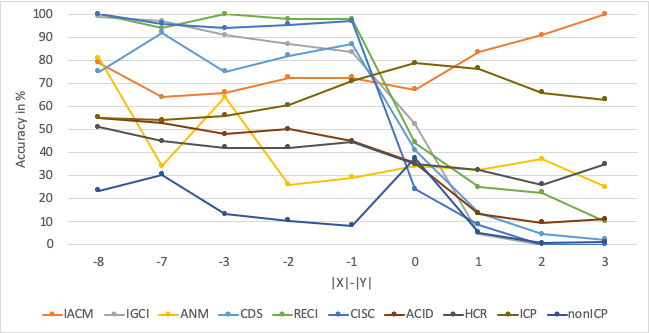
\includegraphics[scale=1.3]{result_linear_discrete.png}
        \subcaption{}
        \label{fig:discrete_linear}
 \end{minipage}
 \hfill
 \begin{minipage}{0.49\linewidth}
\centering
         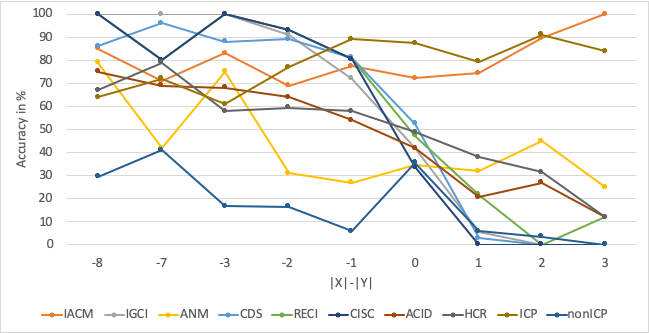
\includegraphics[scale=1.3]{result_nonlin_discrete.png}
        \subcaption{}
        \label{fig:discrete_nonlinear}
       \end{minipage}
       \caption{Averaged accuracies of correct inferred causal direction for linear (a) and nonlinear (b) synthetic data relative to the difference in range size $|\kX| - |\kY|$ for small range sizes.}
       \label{fig.synthetic_results}
 \end{minipage}
\end{figure}

\subsection{Real-World Data}

As a benchmark set consisting of real-world data, we use $102$ manually labeled continuous cause-effect pairs (CEP) from different contexts \cite{MPJZS16, DG19}. As real-world discrete data sets, we use $4$ anonymous discrete cause-effect pairs where food intolerances cause health issues (Food)\footnote{This dataset, given as discrete timeseries data, has been provided by the author and the causal direction has been independently confirmed by medical tests.}, the Pittsburgh bridges dataset (Bridge, $4$ pairs) from \cite{DG19} as it has been used in \cite{CQZZH18}, and the Abalone dataset (Abalone, $3$ pairs) from the UCI Machine Learning Repository \cite{DG19}. For the CEP data set IACM outperforms all other methods. Also for discrete real-world data we can see in Figure \ref{fig.real_world_resultsb} that IACM successfully recovers all causal directions and can keep pace with state-of-the-art methods.

\begin{figure}[htb]
\begin{minipage}{\linewidth}
      \begin{minipage}{0.48\linewidth}
	      \centering
		  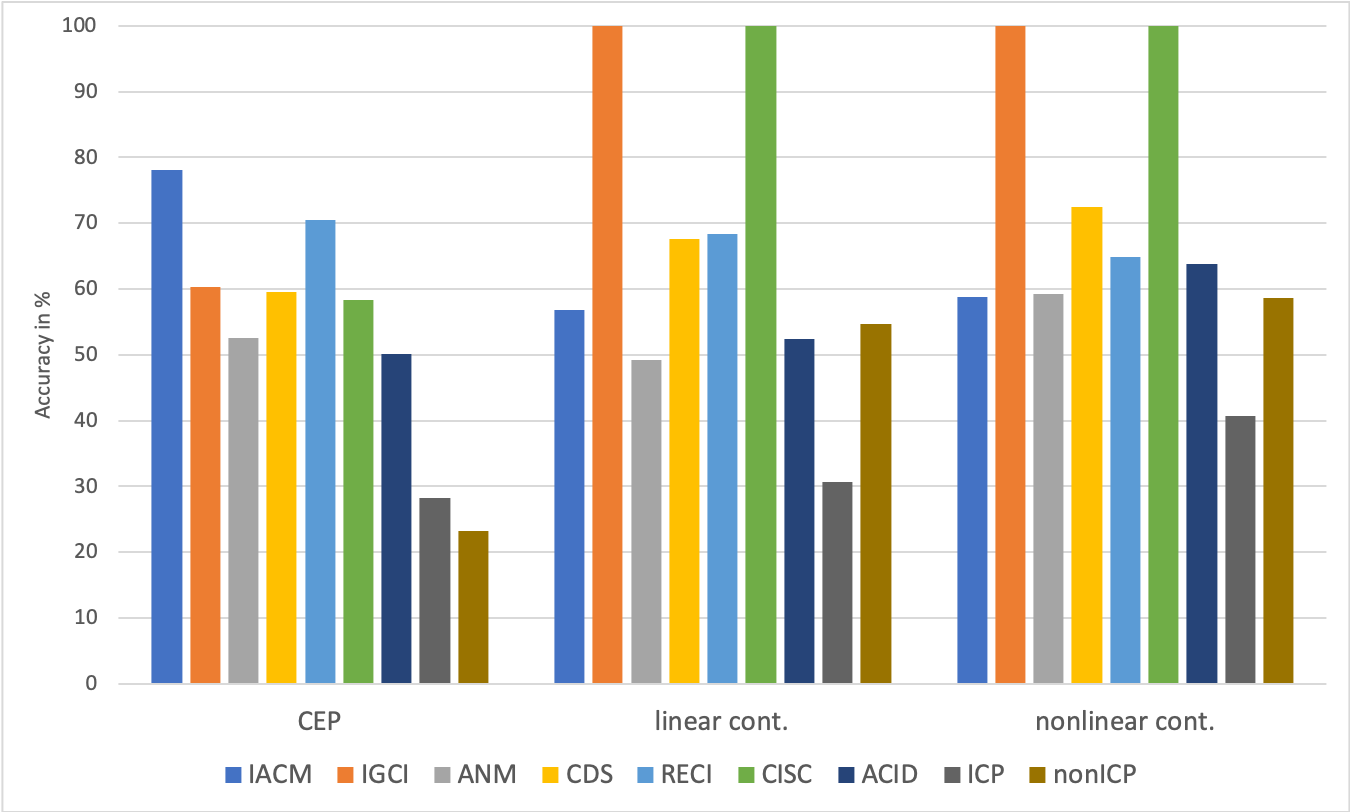
\includegraphics[scale=0.3]{results_cont_data.png}
           \subcaption{Accuracies of synthetic linear and nonlinear continuous data and of continuous real-world data (CEP).}
           \label{fig.real_world_resultsa}
      \end{minipage}
      \hfill
      \begin{minipage}{0.48\linewidth}
	      \centering
  		  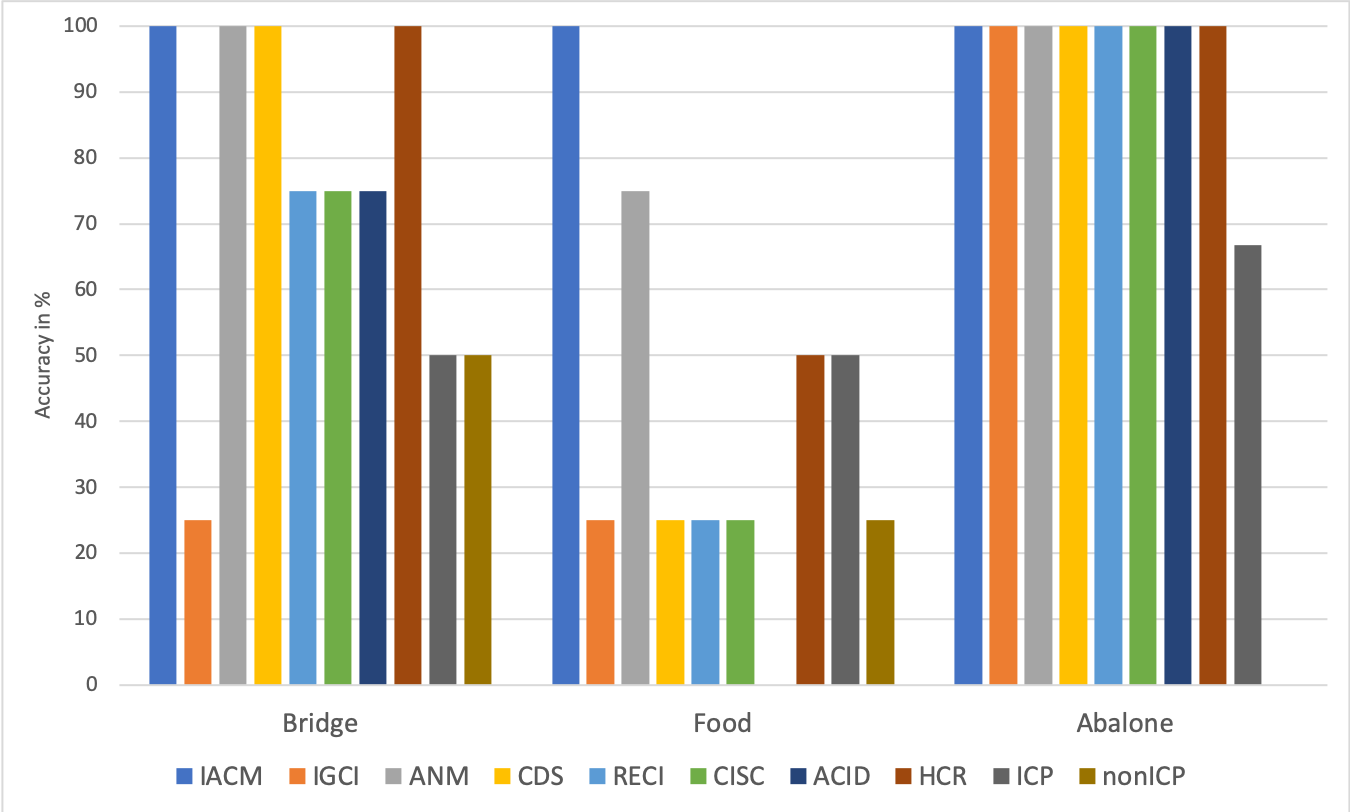
\includegraphics[scale=0.3]{result_real_discrete.png}
           \subcaption{Accuracies of different discrete real-world data sets.}
            \label{fig.real_world_resultsb}
      \end{minipage}
       \caption{Accuracies of correct inferred causal directions for continuous and discrete data.}
  \end{minipage}
\end{figure}

\section{Discussion} \label{sec.discussion}

In this paper, we proposed a way how empirical distributions coming from observations and experiments can be approximated to ones that follow the restrictions enforced by an assumed causal model. This can be used to calculate probabilities of causation and leads to a new causal discovery method. In our experiments, we could confirm that our approach can compete with the current state-of-the-art methods, also on real-world datasets (continuous and discrete) and without the explicit knowledge of experimental data. Especially for the discrete setting in which the range size of the cause is greater than the range size of the effect, our method has advantages compared to other approaches. Since IACM ran with small range sizes $b_x$ and $b_y$, it seems that in many cases the essential cause-effect information can be encoded with much less information than we might have in the data. This is interesting by itself and could serve as a base for future research.

\section*{Broader Impact}

As all methods for causal discovery that use observational and/or data from implicit interventions the work in this paper could help to avoid unethical experiments. Furthermore, it contributes to a more relieable detection of causal relations, since it fills a gap in the existing causal discovery landscape. Therefore, our research can help during the evaluation and design of studies with few discrete features and contribute to more solid conclusions of those studies. On the other hand there is a potential risk that our method is used for data that are not following the assumptions of this paper. This may lead to wrong causal directions and to wrong conclusions, but can be avoided by checking the assumptions on the data before applying our method. Finally, it should be noted that this article may inspire future research projects in the field.

\bibliographystyle{myamsalpha}
\bibliography{mrabbrev, references}

%\section{Supplementary Material}
%
%\subsection{Proof of Lemma \ref{lemma.characterization}}
%\begin{lemma}{\ref{lemma.characterization}}
%The set of joint probability distributions for $X, Y, Y_{a}$, for all $a \in \kX_X$ which fulfill the consistency condition (\ref{consistencyCondition}) is called $\kM_C$ and given as
%\begin{eqnarray*}
%\kM_C & = & \left \{P \in \kP(\kX_V) \mid \pi_{X, Y, Y_{a}} P(a, y, \overline{y}_{a}) = \pi_{X, Y, Y_{a}} P(a, \overline{y}, y_{a}) = 0 \right. \\
%& & \qquad \qquad \qquad \left. \forall \; y \in \kX_Y, y_{a} \in \kX_{Y_{a}}, a \in \kX_X \right \},
%\end{eqnarray*}
%where $\overline{y}_{a} \in \kX_{Y_{a}} \backslash \{y_{a}\}$ for $a \in \kX_X$ and $\overline{y} \in \kX_Y \backslash \{y\}$.
%\end{lemma}
%\begin{Proof}
%The consistency condition (\ref{consistencyCondition}) implies the following relation for some $P \in \kP(\kX_V)$ and $a\in \kX_X$
%\begin{eqnarray*}
%\pi_{X, Y} P(a, y) & = & \pi_{X, Y, Y_{a}} P(a, y, y_{a}), \qquad {\rm with} \; y=y_{a}.
%\end{eqnarray*}
%These relation implies
%\begin{eqnarray*}
%\pi_{X, Y, Y_{a}} P(a, y, \overline{y}_{a}) = \pi_{X, Y, Y_{a}} P(a, \overline{y}, y_{a}) = 0, {\rm \;for}\;a \in\kX_X,
%\end{eqnarray*}
%which characterizes the joint distributions that satisfy (\ref{consistencyCondition}).
%\end{Proof}
%
%\subsection{Proof of Proposition \ref{prop.approx_solution}}
%
%\begin{satz}{\ref{prop.approx_solution}}
%The optimization problem (\ref{equ.MinMinProblem}) simplifies to the following linear optimization problem
%$$
%\max_{\substack{\hat P \in \kP(\kX_V),\\ \pi_{X,Y} \hat P = P_{XY}, \pi_{Y_{a}} \hat P = P_{Y_{a}},a\in \kX_X}} S(\hat P),
%$$
%with $S(\hat P):= \sum_{z \in \supp(\kM_C)} \hat P(z)$.
%\end{satz}
%\begin{Proof}
%We first consider the inner minimization problem of (\ref{equ.MinMinProblem}) for a given joint distribution $\hat P \in \kP(\kX_V)$. This is a constrained optimization problem where the constraints in $\kM_C$ are equivalent to the equation
%$$
%S(\tilde P) = 1,
%$$
%since $\tilde P$ is a probability distribution. Therefore, the Lagrange functional of this minimization problem reads
%$$
%\Lambda(\tilde P) := D(\hat P || \tilde P) + \lambda \left (S(\tilde P) - 1
%\right ),
%$$
%with $\lambda$ as Lagrange multiplier. Using the Lagrange multiplier method we obtain explicit expressions for the approximating distribution $\tilde P \in \kM_C$
%$$
%\tilde P (z)= \frac{\hat P(z)}{S(\hat P)}
%$$
%for $z \in \supp(\kM_C)$ and $\tilde P(z) = 0$ for all $z \notin \supp(\kM_C)$. Thus we have solved the inner minimization problem explicitly and the relative entropy simplifies to
%$$
%D( \hat P || \tilde P) = - \log(S( \hat P)).
%$$
%Therefore, we can now optimize on the space of possible joint distributions and (\ref{equ.MinMinProblem}) simplifies to
%$$
%\max_{\substack{\hat P \in \kP(\kX_V),\\ \pi_{X,Y}\hat P = P_{XY}, \pi_{Y_{a}} \hat P = P_{Y_{a}},a\in \kX_X}} \log(S(\hat P)).
%$$
%Since $\log$ is a monotone function it suffices to maximize $S(\hat P)$ given the constraints. But this is nothing than a linear optimization problem which can be solved by linear programming using the simplex algorithm, see, for example, \cite{CLRS01}.
%\end{Proof}
%
%\subsection{Application to Timeseries Data}
%
%Algorithm \ref{alg.approximationAlgo} can also be applied when we assume that the underlying causal model has a time lag of $T$, which is $X_{t-T} \rightarrow Y_t$, and the observational and interventional data have a time order. We only have to shift the incoming data for $X_t$ and $Y_t$ so that Algorithm \ref{alg.approximationAlgo} applies to $X_{t}, Y_{t+T}$, and has to take care that we preserve the data order during preprocessing steps. If we do not know the exact time lag we can run the approximation several times with different time lags to find
%the approximation with the lowest error. 
%
%\subsection{Data Preprocessing}
%
%Algorithm \ref{alg.iacmdiscovery} includes several preprocessing steps for sample data from $X$ and $Y$ that can be parametrized. The preprocessing steps split the data into obersvational data and interventional data for $X$ and $Y$ accordingly. These steps are:
%\begin{itemize}
%	\item \code{discrete-cluster}: discretize data from $X$ and $Y$ using \code{KBinsDiscretizer} to a number of bins. Apply a $k$-means clustering to the discretized data with fixed number of clusters. We split the data according to the variance in the identified cluster. If $X$ is the assumed cause, then the cluster with the lowest variance in $X$ determines the observed data and the union of the other clusters the interventional data. 
%	\item \code{cluster-discrete}: the steps of \code{discrete-cluster} are interchanged. The data are first clustered, then discretized, and split according the variance in the clusters.
%\end{itemize}
%
%\subsection{Parameter Setting in Experiments}
%
%In the experimental runs we used the following parameter configuration to run IACM. If $|\kX|=2, |\kY|<5$ or $|\kX|<5, |\kY|=2$ we used no preprocessing, since the binary discretization build into IACM itself provides a good job. If $|\kX|-|\kY| < 0$ we used \code{discrete-cluster} as preprocessing and used $D(\pi_X \hat P || \pi_Y \hat P)$ as a decision criterion for the causal direction. In the other case when $|\kX|-|\kY| \ge 0$ we used \code{discrete-cluster} but $-\log(S(\hat P))$ as decision criterion. For data with continuous or large range sizes we used \code{cluster-discrete} as preprocessing and the approximation error as decision criterion. The number of bins and cluster used in the discretization and clustering part is choosen such that is near to the range size of the data. Our experiments also show that this heuristics defining the meta parameters for IACM is by far not optimal. We left that for future research.

\end{document}
